\documentclass{article}

\usepackage{amsmath}
\usepackage{gensymb}
\usepackage{graphicx}
\usepackage{caption}

\title{On the Use of Solar in Hydrogen Generation and Fuel Cells}
\author{Elliott Ashby}
\date{\today}

\begin{document}
    \maketitle
    \begin{thebibliography}{3}
        \bibitem{SCE}
        Department of Physics: University of Southampton \emph{Solar Cells extension - Hydrogen Electrolyser and Fuel Cell instructions}
        \bibitem{P:SE}
        Department of Physics: University of Southampton \emph{Production: Solar Energy}
        \bibitem{ETH}
        Averil Macdonoald \& Martyn Berry \emph{Energy through Hydrogen}, heliocentris
    \end{thebibliography}
    \section{Introduction}

    This project will investigate and document the properties and characteristics
    of energy generation and conversion using the \(\text{Hydro-Genius}^{\text{TM}}\)Professional module (\textbf{Figure 1}), 
    which contains a solar cell, a water splitting cell in order to generate hydrogen and 
    a hydrogen fuel cell. This project aims to provide it's author with an understanding 
    of the fundamentals in the solar hydrogen technology space in addition to explaining 
    why solar hydrogen is a suitable form of sustainable energy for the future. As seen in \textbf{Figure 4}.
    \begin{figure}
        \centering
        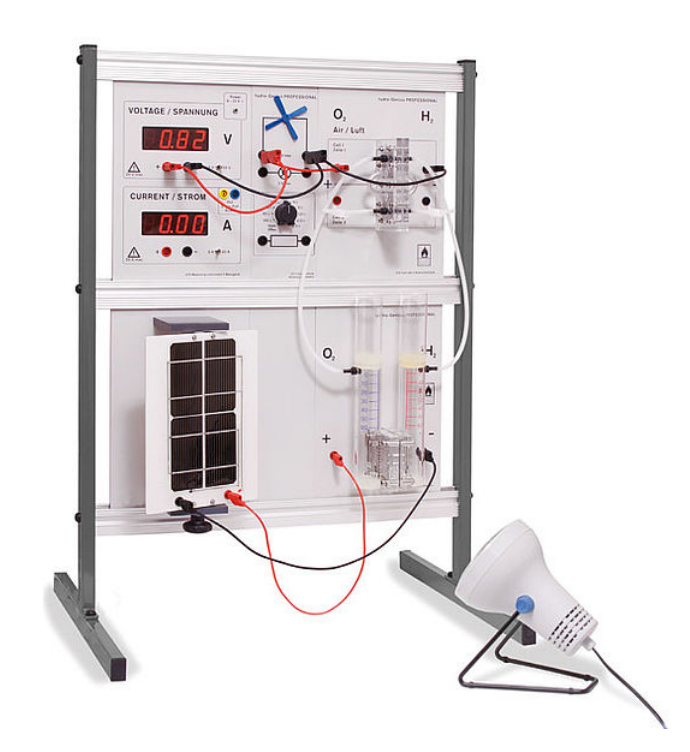
\includegraphics[scale=0.3]{./module.png}
        \caption{\(\text{Hydro-Genius}^{\text{TM}}\)\cite{SCE}}
    \end{figure}

    \subsection{Aim}
        The projects aims are listed below:
        \begin{itemize}
            \item succeeding that, using the solar energy generated to record the characteristic response and efficency 
            of the hydrogen generated, and finally,
            \item investigate the characteristic response of the solar cell, both under illumination and in the dark,
            \item to characterize a hydrogen fuel cell's energy conversion.
        \end{itemize} 
    \section{Theory}
    \subsection{Production of electricity through solar energy}
    \begin{itemize}
        \item Photovotaic panels convert some frequencies of electromagnetic radiation into and electric current.
        \item These PV panels (see \textbf{Figure 5}) create higher-grade electrical energy compared to thermal solar panels
    \end{itemize}
    The Photovotaic Effect
    \begin{itemize}
        \item Crystalline semi-conductors are composed of atoms and electrons bound in a lattice.
        \item If an electron in the lattice gains enough energy, it is radicalized from the lattice and can move, creating a current.
        \item In photovotaic materials this process can be performed through electrons absorbing electromagnetic radiation.
        \item The crystalline lattice can be 'doped' using other elements to change how it interacts with these free electrons that fall into
        two catagories, wither positive (p) or negative (n) carriers.
        \newpage
        \item For silicon (group IV):
            \begin{itemize}
                \item P-type: Boron (group III)
                \item N-type: Phosphorus (group V)
            \end{itemize}
        \item These p and n type semiconductors can be placed next to one another to create pn junctions (see \textbf{Figure 6}).
        \item By creating a pn junction, carriers at the interface recombine forming the labeled 'Space Charge Region' also known as the 'depletion layer'.
        \item The width of the depletion layer can additionally be controlled by applying an external voltage. This is called the diode-effect.
        \item The IV-curve of the pn-junction (diode) is called the Shockley equation
        \begin{equation}
            I_D = I_S (e^{\frac{qV_D}{nkT}}-1)
        \end{equation}
        where \(I_D \text{ and } V_D\) are the diode and voltage respectively, q is the charge on the electron, 
        n is the ideality factor: n=1 fro indirect semiconductors or n=2 for direct semiconductors, k is Boltzmann's constant, T is temperature in kelvin, 
        \(\frac{kT}{q} \text{ is also known as } V_{th}\), the thermal voltage.
        \item Under illumination the solar cell follows the Shockley equation but vertically shifted by the photocurrent.
    \end{itemize}
    \subsection{Water electrolysis using solid electrolyte membranes}
    In order to electrolyse water, electrodes must be separated by a membrane preventing gases from mixing 
    and creating and explosive combination of hydrogen and oxygen, but still requires ions to pass through it. 
    In order to keep electrical resistance low, the electrodes and solid electrolyte membrane are in extremeley close contact. 
    \newline
    \begin{itemize}
        \item The theoretical voltage required for splitting water into its constituent components is 1.23V. 
        However, in practice, there is waste energy and therefore the usual voltage has to be higher then 1.23V. 
        Good electrode and catalyst design can bring the voltage required down to 1.7 - 1.9V and the closer the operating 
        voltage is to the theoretical minimum voltage, the greater the efficency of the process along with a lower waste of energy.
        \item \textbf{Figure 2} shows an alkaline electrolyser. At it's anode, hydroxide ions give up their extra electrons and are 
        oxidised to oxygen and water. At the cathode, water is instead reduced to hydrogen and hydrogen ions. This completes the 
        circuit since hydroxide ions passing through the membrane from the cathode pass through to the anode side.
    \end{itemize}
    At the anode: \cite{ETH}
    \begin{equation}
        4OH^-(aq)\rightarrow O_2(g) + 2H_2O(l) + 4e^-
    \end{equation}
    At the cathode: \cite{ETH}
    \begin{equation}
        4H_2O(l) + 4e^- \rightarrow 2H_2(g) + 4OH^-(aq) 
    \end{equation}
    Overall: \cite{ETH}
    \begin{equation}
        2H_2O(l) \rightarrow 2H_2(g) + O_2(g)
    \end{equation}
    \begin{figure}
        \centering
        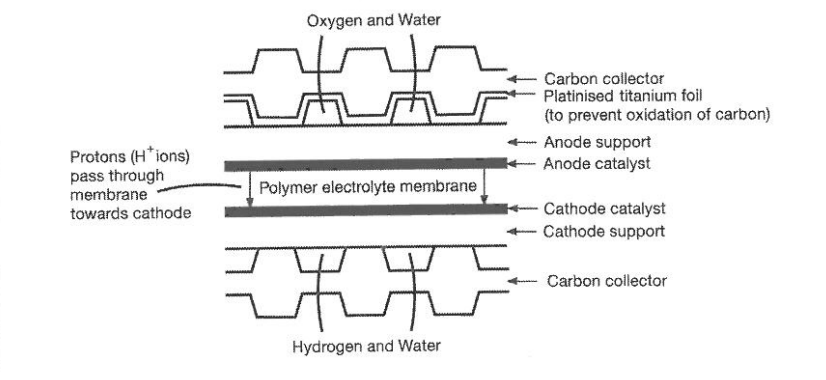
\includegraphics[scale=0.4]{./electro.png}
        \caption{Schematic diagram of an alkaline electrolyser \cite{ETH}}
    \end{figure}
    \subsection{Fuel cells}
    A basic hydrogen fuel cell (see \textbf{Figure 3}) consists of two porous carbon cloth electrodes bonded to a polymer electrolyte membrane. 
    Outside the electrodes are flow field plates. These contain channels to ensure that the gases are in contact with the whole surface 
    of the electrodes. They also serve to remove the water which is produced.
    \newline Oxidation occurs at the anode and reduction at the cathode. The fuel, hydrogen, is oxydised at the anode 
    and releases electrons. These electrons flow from the anode around the circuit to the cathode. Hydrogen ions flow through 
    the polymer electrolyte membrane to the cathode to balance the charges. \cite{ETH}
    \newline The reactions are hence:
    \newline At the anode: \cite{ETH}
    \begin{equation}
        2H_2(g) \rightarrow 4H^+ + 4e^-
    \end{equation}
    At the cathode: \cite{ETH}
    \begin{equation}
        O_2(g) + 4H^+ + 4e^- \rightarrow 2H_2O(l)
    \end{equation}
    Overall: \cite{ETH}
    \begin{equation}
        2H_2(g) + O_2(g) \rightarrow 2H_2O(l)
    \end{equation}
    A hydrogen fuel cell has a maximum theoretical output voltage of 1.23V since the potential is the same as the decomposition of water. However 
    in practice, becuase of various losses in efficency, such as back reaction, internal resistance and bad diffusion of gases, typically a good voltage 
    will be between 0.6 and 0.9V.
    \newline Higher voltages can be easily obatained by connected fuel cells in series in what are called 'stacks'.
    \begin{figure}
        \centering
        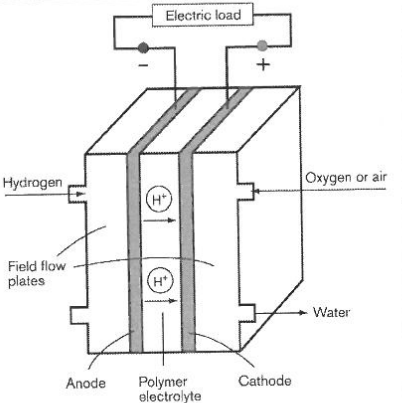
\includegraphics[scale=0.4]{./fuel.png}
        \caption{The arrangement in a typical hydrogen fuel cell \cite{ETH}}
    \end{figure}
    \section{Apparatus}
    The \(\text{Hydro-Genius}^{\text{TM}}\)module which contains:
    \begin{itemize}
        \item Electrolyser
        \item Fuel Cells
        \item Load (resistance) module
        \item Ammeter
        \item Voltmeter
        \item Solar module
    \end{itemize}
    In addition, leads (to connect the apparatus into the circuits required), tubes (for directed water transportation), 
    a fan (for cooling the solar cell), a lamp (100-150 Watt), and distilled water (tap water contains higher proportions of minerals 
    and impurities), are required to carry out the experiments.
    \subsection{Apparatus Notes}
    In order to maintain good operation of the module and it's components the following notes should be observed:
    \begin{itemize}
        \item Only distilled water should be used, as other liquids may cause corrosion and damage to the intruments.
        \item The solar module should stay below \(60^\circ C\) otherwise damage may be caused to the solar cells or melt the plastic 
        parts.
        \item Any voltage \(>\) 3.5 Volts connected to the modules could cause damage to the instruments and as such no external power supplies 
        with voltage output \(>\) 3.5 Volts should be connected.
    \end{itemize}
    \begin{figure}
        \centering
        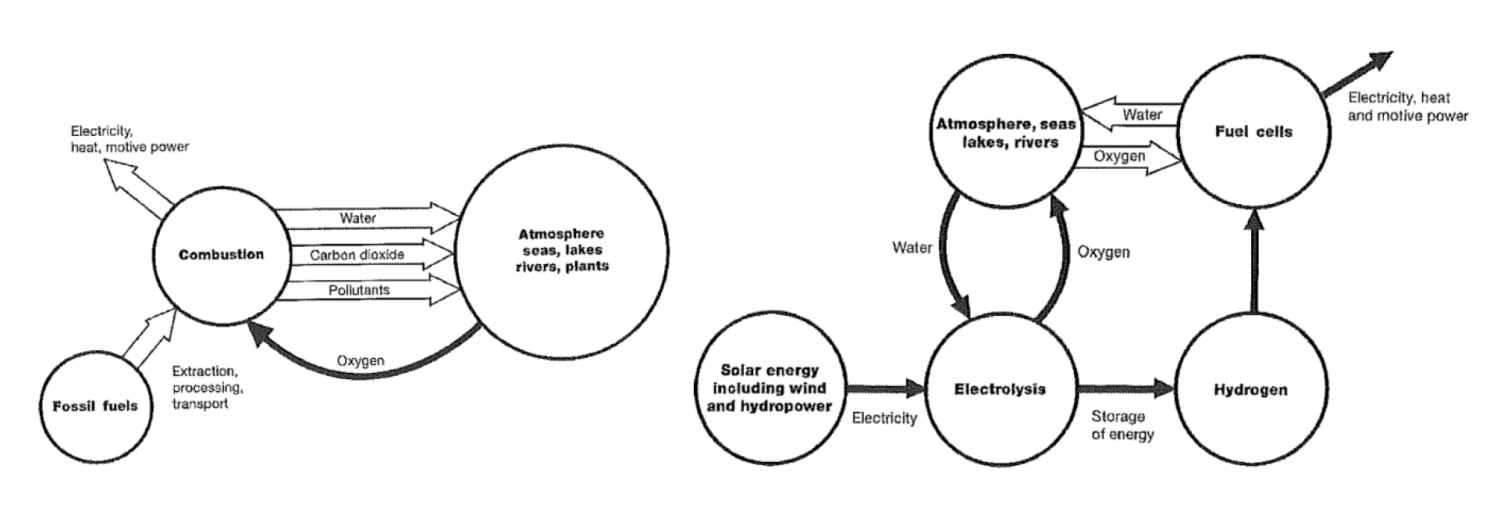
\includegraphics[scale=0.25]{./cycle.png}
        \caption{(left) Fossil fuels: main source of energy present, depletion is inevitable. (right) 
        Probable supply of energy in the future through hydrogen: the loop is closed, and the supply can be maintained 
        as long as the sun remains in a steady state. \cite{SCE}}
    \end{figure}
    \subsection{Safety}
    The experiments will produce both oxygen (\(O_2\)) and hydrogen (\(H_2\)), which will be contained within the module 
    and should pose no risk under normal circumstances and in small amounts. Most notably, ignition sources should be 
    kept at distance to prevent ignition of either the oxygen or the hydrogen when using the electrolyser.
    \newline The solar module will become hot when absorbing radiation from the lamp. In the instances when the solar cells 
    are hot, refrain from touching them. A temperature sensor can be used to monitor the temperature of the unit. 
    Make sure the temperature does not exceed \(60^{\circ}C\) By keeping the lamp a good distance from the solar module.
    \begin{figure}
        \centering
        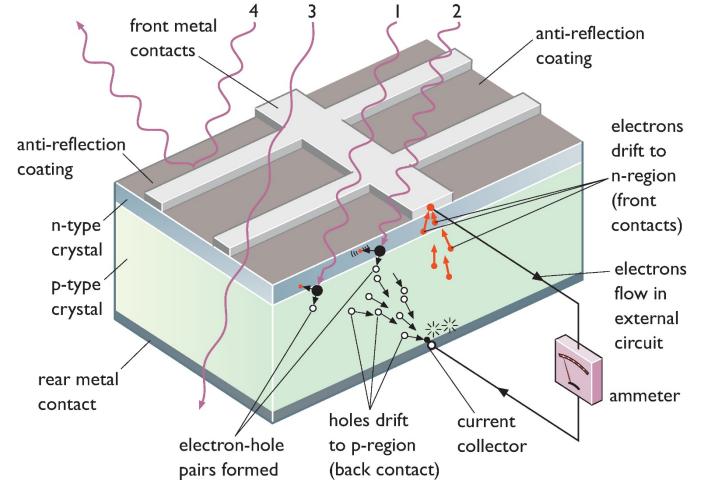
\includegraphics[scale=0.4]{./cell.png}
        \caption{PV solar panel cross section. \cite{P:SE}}
    \end{figure}
    \section{Methods}
    \subsection{Investigating the electrolysis of water}
    \begin{enumerate}
        \item Set up the apparatus like in \textbf{Figure 7}, making sure the correct terminals are connected.
        \item Vary the light intesity to adjust the current generated by the solar cell. This can be done most easily 
        rotating the solar module at different angles to the lamp. Set different values of current, approximately 30mA to 
        800mA and record the voltage across the electrolyser.
    \end{enumerate}
    \begin{figure}
        \centering
        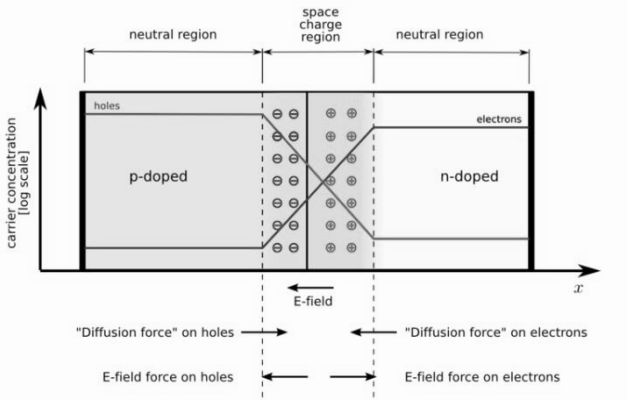
\includegraphics[scale=0.4]{./pn.png}
        \caption{pn junction as used in solar cells. \cite{P:SE}}
    \end{figure}
    \begin{figure}
        \centering
        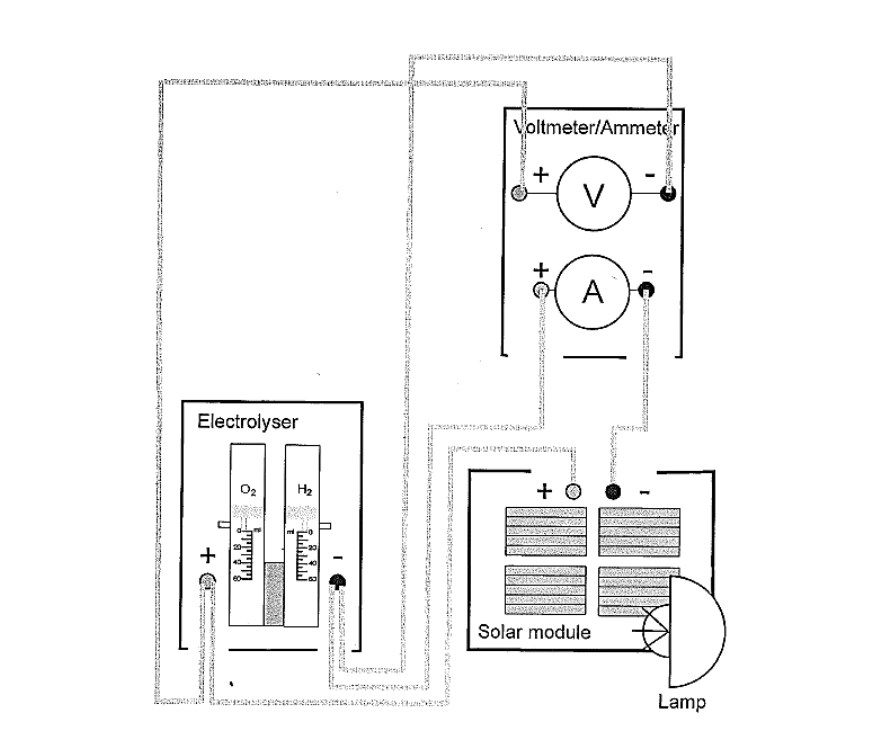
\includegraphics[scale=0.3]{./three.png}
        \caption{Setup for the electrolysis of water experiment. \cite{SCE}}
    \end{figure}
    \subsection{Fuel cell}
    \subsubsection{Current-voltage characteristics of the fuel cell}
    This experiment will use the energy stored in the hydrogen to power a hydrogen fuel cell which works through reverse 
    electrolysis, combining the oxygen and hydrogen to produce electricity and water.
    \begin{enumerate}
        \item  The fuel cell, in order to produce electricity and water, needs a supply of hydrogen and oxygen from the 
        electrolyser (see \textbf{Figure 8}). Make sure the tubes are correctly connected.
        \item Rotate load resistor to the 'OPEN' position.
        \item The gas storage cyclinders should be filled to the 0ml mark. Using the solar module, set a constant current 
        to the electrolyser of between 200 and 300 mA.
        \item Purge the system for 5 minutes with the produced gases. Then rotate the load resistor to 3 ohms for 3 minutes. 
        The ammeter should show a current being produced. Purge the system again with the load resistor at the 'OPEN' position.
        \item Stop the power supply briefly and use the tube clips to close the two shorter tubes on the lower half of the fuel cell.
        \item Reconnect the power supply to the electrolyser and store the gases in the gas storage cyclinders. Interrupt the power 
        supply when the hydrogen side of the electrolyser reaches the 10ml mark.
        \item Record the characteristic curve of the fuel cell by varying the measurement resistance. Start at the 'OPEN' position, 
        then measure the volatage and current at each resistance level. Additionally measure the volatage and current for the lamp 
        and the electric motor.
    \end{enumerate}
    \begin{figure}
        \centering
        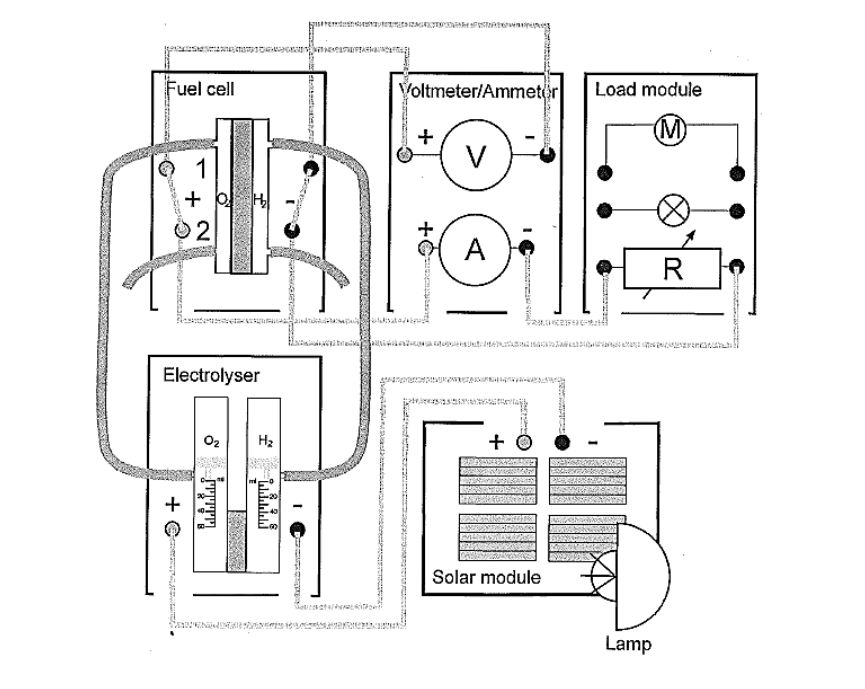
\includegraphics[scale=0.3]{./four.png}
        \caption{Setup for fuel cell experiment. \cite{SCE}}
    \end{figure}
    \section{Results and Analysis}
    
    \section{Conclusions}
\end{document}